%%%%%%%%%%%%%%%%%%%%%%
% Wenneker Resume/CV %
%%%%%%%%%%%%%%%%%%%%%%
\documentclass[a4paper,12pt]{memoir} % Font and paper size

\usepackage{multirow}
\input{structure.tex} % Include the file specifying document layout and packages

%----------------------------------------------------------------------------------------
%	NAME AND CONTACT INFORMATION
%----------------------------------------------------------------------------------------

\userinformation{ % Set the content that goes into the sidebar of each page
\begin{flushright}
% Comment out this figure block if you don't want a photo
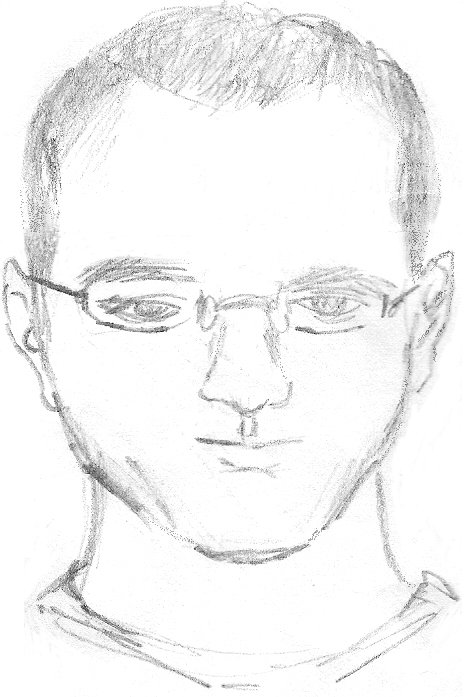
\includegraphics[width=\columnwidth]{lex.png}\\[\baselineskip] % Your photo
\large \textbf{Alex Towell} \\
\small \href{mailto:lex@metafunctor.com}{lex@metafunctor.com} \\
\vspace{0.5cm}
\href{https://metafunctor.com}{metafunctor.com} \\
\href{https://github.com/queelius}{github.com/queelius} \\
\vspace{0.5cm}
(618) 977-1746 \\ % Your phone number
\vfill % Whitespace under this block to push it up under the photo
\end{flushright}
}


%----------------------------------------------------------------------------------------

\begin{document}

\userinformation % Print your information in the left column

\framebreak % End of the first column

%----------------------------------------------------------------------------------------
%	HEADING
%----------------------------------------------------------------------------------------

\cvheading{Alex Towell} % Large heading - your name

\cvsubheading{PhD Student | Mechanistic Interpretability | AI Safety}

%----------------------------------------------------------------------------------------
%	ABOUT ME
%----------------------------------------------------------------------------------------

\aboutme{About Me}{Computer Science PhD student with dual master's degrees (CS \& Mathematics/Statistics) seeking to understand how neural networks represent and process information. Recent work applies network analysis to AI conversations, revealing hidden cognitive structure---directly analogous to circuit analysis in neural networks. I value reproducibility, systematic evaluation, and honest uncertainty quantification.}

%----------------------------------------------------------------------------------------
%	PUBLICATIONS
%----------------------------------------------------------------------------------------

\CVSection{Publications}

\begin{itemize}
    \item \textbf{A. Towell}, J. Matta, ``Cognitive MRI of AI Conversations: Analyzing AI Interactions through Semantic Embedding Networks,'' \textit{Complex Networks \& Their Applications (CNA)}, 2025
    \item H. Fujinoki, \textbf{A. Towell}, V.A. Thota, ``Preventing Ransomware Damages using In-Operation Off-Site Backup to Achieve a $10^{-8}$ False-Negative Miss-Detection Rate,'' \textit{ICCCI}, 2025
    \item \textbf{A. Towell}, ``Reliability Estimation in Series Systems,'' Master's Project, SIUE, 2023
    \item \textbf{A. Towell}, H. Fujinoki, ``Estimating How Confidential Encrypted Searches Are,'' \textit{IEEE CloudCom}, 2016
\end{itemize}

\Sep

%----------------------------------------------------------------------------------------
%	EDUCATION
%----------------------------------------------------------------------------------------

\CVSection{Education}

\CVItem{2024 - Present, Southern Illinois University}{PhD in Computer Science}
{Focus: AI Safety, Interpretability, Network Analysis. Advisor: Dr. Hiroshi Fujinoki}

\SmallSep

\CVItem{2021 - 2023, SIUE}{MS in Mathematics (GPA: 3.9/4.0)}
{Concentration: Statistics and Operations Research}

\SmallSep

\CVItem{2012 - 2015, SIUE}{MS in Computer Science (GPA: 4.0/4.0)}
{Concentration: Artificial Intelligence. Outstanding Graduate Student Award.}

\SmallSep

\CVItem{2006 - 2010, SIUE}{BS in Computer Science (GPA: 3.6/4.0)}{}

\Sep

%----------------------------------------------------------------------------------------
% TECHNICAL SKILLS
%----------------------------------------------------------------------------------------

\CVSection{Technical Skills}

\CVItem{Languages}{Python (primary), R, C/C++, TypeScript, Bash, LaTeX}\\
\CVItem{ML/DL}{PyTorch, HuggingFace Transformers, NumPy, Pandas, NetworkX}\\
\CVItem{Methods}{Graph/network analysis, statistical inference, ablation studies}\\

\clearpage % Start a new page

%----------------------------------------------------------------------------------------
% PAGE 2
%----------------------------------------------------------------------------------------

\userinformation % Print your information in the left column

\framebreak

%----------------------------------------------------------------------------------------
% RELEVANT RESEARCH & PROJECTS
%----------------------------------------------------------------------------------------

\CVSection{Relevant Research \& Projects}

\CVItem{Cognitive MRI of AI Conversations (CNA 2025)}{Applied complex network analysis to 449 ChatGPT conversations to reveal latent cognitive structure. Identified heterogeneous topology and three distinct bridge types. Comprehensive ablation study across 63 parameter configurations.}\\
\CVItem{elasticsearch-lm: LLM Fine-Tuning for Query Generation}{Fine-tuning TinyLlama to translate natural language to Elasticsearch queries. Synthetic data generation, evaluation on populated databases. PyPI published, 36+ GitHub stars.}\\
\CVItem{Ransomware Detection}{Detection system achieving $10^{-8}$ false-negative rate using Bloom filters with rigorous statistical evaluation.}\\
\CVItem{Fisher Flow}{Natural gradient descent using Fisher information matrix and information geometry.}\\
\CVItem{Oblivious Computing}{Bernoulli types for principled approximation; algebraic cipher types for homomorphic computation; encrypted search with information-theoretic bounds.}

\Sep

%----------------------------------------------------------------------------------------
% WHY MECHANISTIC INTERPRETABILITY
%----------------------------------------------------------------------------------------

\CVSection{Why Mechanistic Interpretability}

\begin{itemize}
    \item \textbf{Cognitive MRI work}: Network analysis methods to reveal hidden structure in AI conversations---directly analogous to circuit analysis in neural networks
    \item \textbf{Mathematical foundations}: MS in Mathematics with focus on probability, statistics, and analysis
    \item \textbf{Systematic evaluation}: All my research emphasizes ablation studies, uncertainty quantification, and reproducible methodology
    \item \textbf{Implementation depth}: FemtoGrad and similar projects demonstrate understanding systems at the implementation level
\end{itemize}

\Sep

%----------------------------------------------------------------------------------------
% ACADEMIC EXPERIENCE
%----------------------------------------------------------------------------------------

\CVSection{Academic Experience}

\CVItem{2024--Present, Research Assistant, SIU}{
    \begin{itemize}
        \item Network analysis of AI systems with Dr. John Matta (Cognitive MRI paper)
        \item Cybersecurity research with Dr. Hiroshi Fujinoki on adversarial robustness
        \item Lead developer for IDOT D8 traffic monitoring infrastructure
    \end{itemize}
}

\SmallSep

\CVItem{2012--2015, Research/Teaching Assistant, SIUE}{
    \begin{itemize}
        \item AI/ML research on privacy-preserving search and encrypted computation
        \item Taught undergraduate computer science laboratories
    \end{itemize}
}

\end{document}
